\tocless\subsubsection{Perceptron Learning - Artificial Neuron}
In our ANN, a perceptron is an artificial neuron.
It is called an artificial neuron because it is a bio-inspired neuron which models
a neuron in the human brain in terms of inputs and output.

In perceptron learning, we can take two inputs which are put towards an
activation function with a bias attached as seen in Figure \ref{fig:perceptron}.
These inputs are multiplied by the weights that connect the input to the
activation function and depending on the result, the activation function may
fire an output. These inputs are either 1 or -1.

\begin{figure}[h]
	\centering
     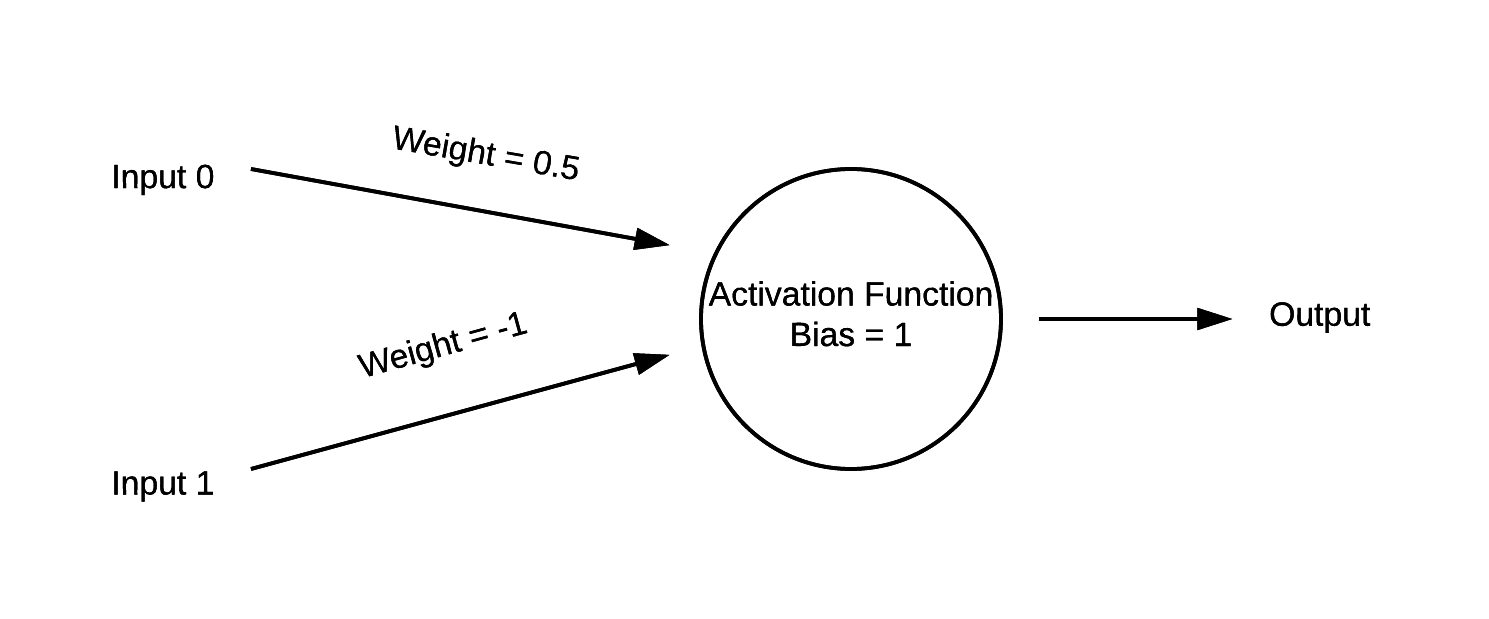
\includegraphics{Perceptron}
     \caption{Perceptron}
     \label{fig:perceptron}
\end{figure}

The Perceptron Training Rule is how weights are selected to produce the correct output during training.
As in \parencite{MLANN}, a common way to train a perceptron is to start with random weights and change them during training as per the training rule.
This rule follows the formula in Equation \ref{eqn:perceptron1}, where xi is the input and Equation \ref{eqn:perceptron2} is valid:
\begin{equation}\label{eqn:perceptron1}
    w_{i} \leftarrow w_{i} + \Delta w_{i}
\end{equation}

\begin{equation}\label{eqn:perceptron2}
    \Delta w_{i} = n(t-o)x_{i}
\end{equation}

In Equation \ref{eqn:perceptron2}, "t is the target output for the current training example, o is the output generated by the perceptron, and n is the positive constant called the learning rate" \parencite{MLANN}.
The output of a neuron is calculated using the activation function.
This Perceptron Training Rule assumes that there are two sets of instances, a
positive and negative set (class x and - in Figure \ref{fig:ls}), and that they are linearly separable, as in demonstrated in Figure \ref{fig:ls}. 

\begin{figure}[h]
	\centering
    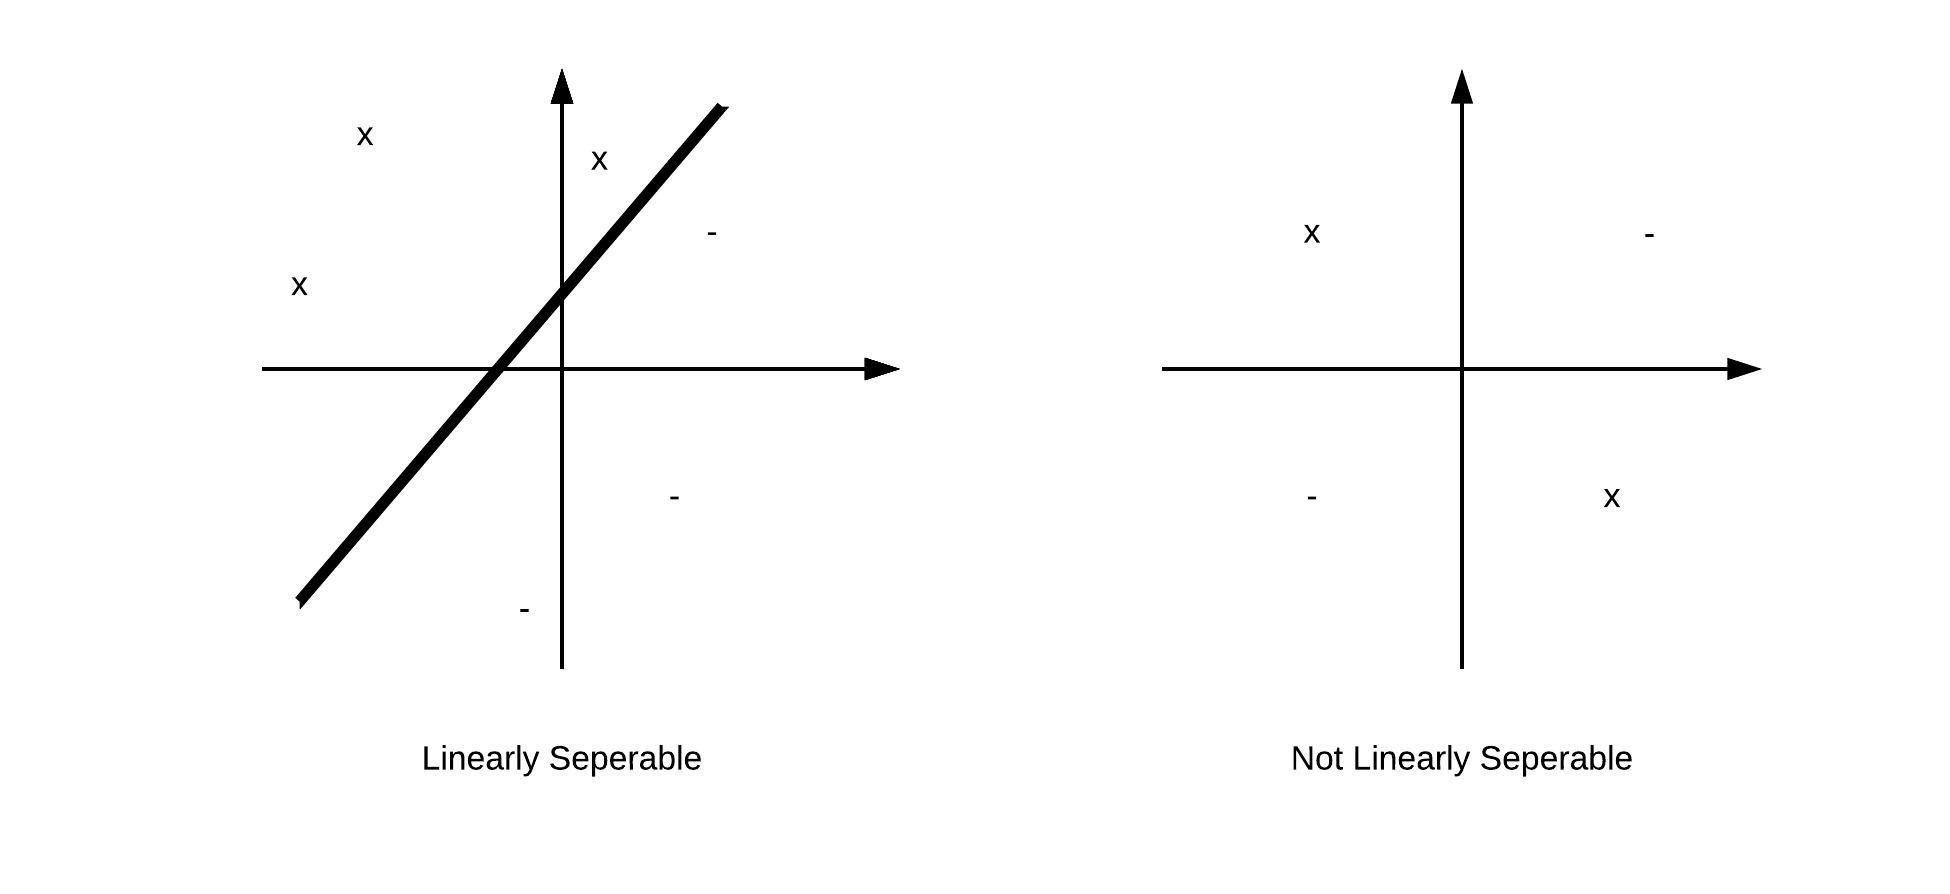
\includegraphics{LS}
     \caption{Linearly Separable, adapted from \parencite{MLANN}}
     \label{fig:ls}
\end{figure}

A perceptron is trained using supervised learning. When the perceptron
classifies a result, it is told if it is correct or not. If the result is
incorrect, weights are changed in value so that this error can be reduced
\parencite{AI}. 

There is one major problem with perceptron learning and that is, it can't solve
a problem if there is not a clear linear separation between the classes. There
is a way in which we can attempt to solve this, through the delta rule. The
delta rule utilises gradient descent to find the best weight for the training
samples \parencite{MLANN}. We will discuss gradient descent in the next section.

\tocless\subsubsection{Multi Layered Perceptron}
Multi-Layer Perceptrons (MLPs) are made up of multiple layers of perceptrons connected
together and are used to combat non-linearly separable classes.
While the delta rule can solve problems of non-linearity when there are two classes, MLPs can solve non-linearity when there are more than two classes.
Firstly, we have an input layer, followed by one or more hidden layers and then
finally an output layer.
Any ANN with more than three hidden layers is categorised as a deep neural network.

\begin{figure}[h]
	\centering
    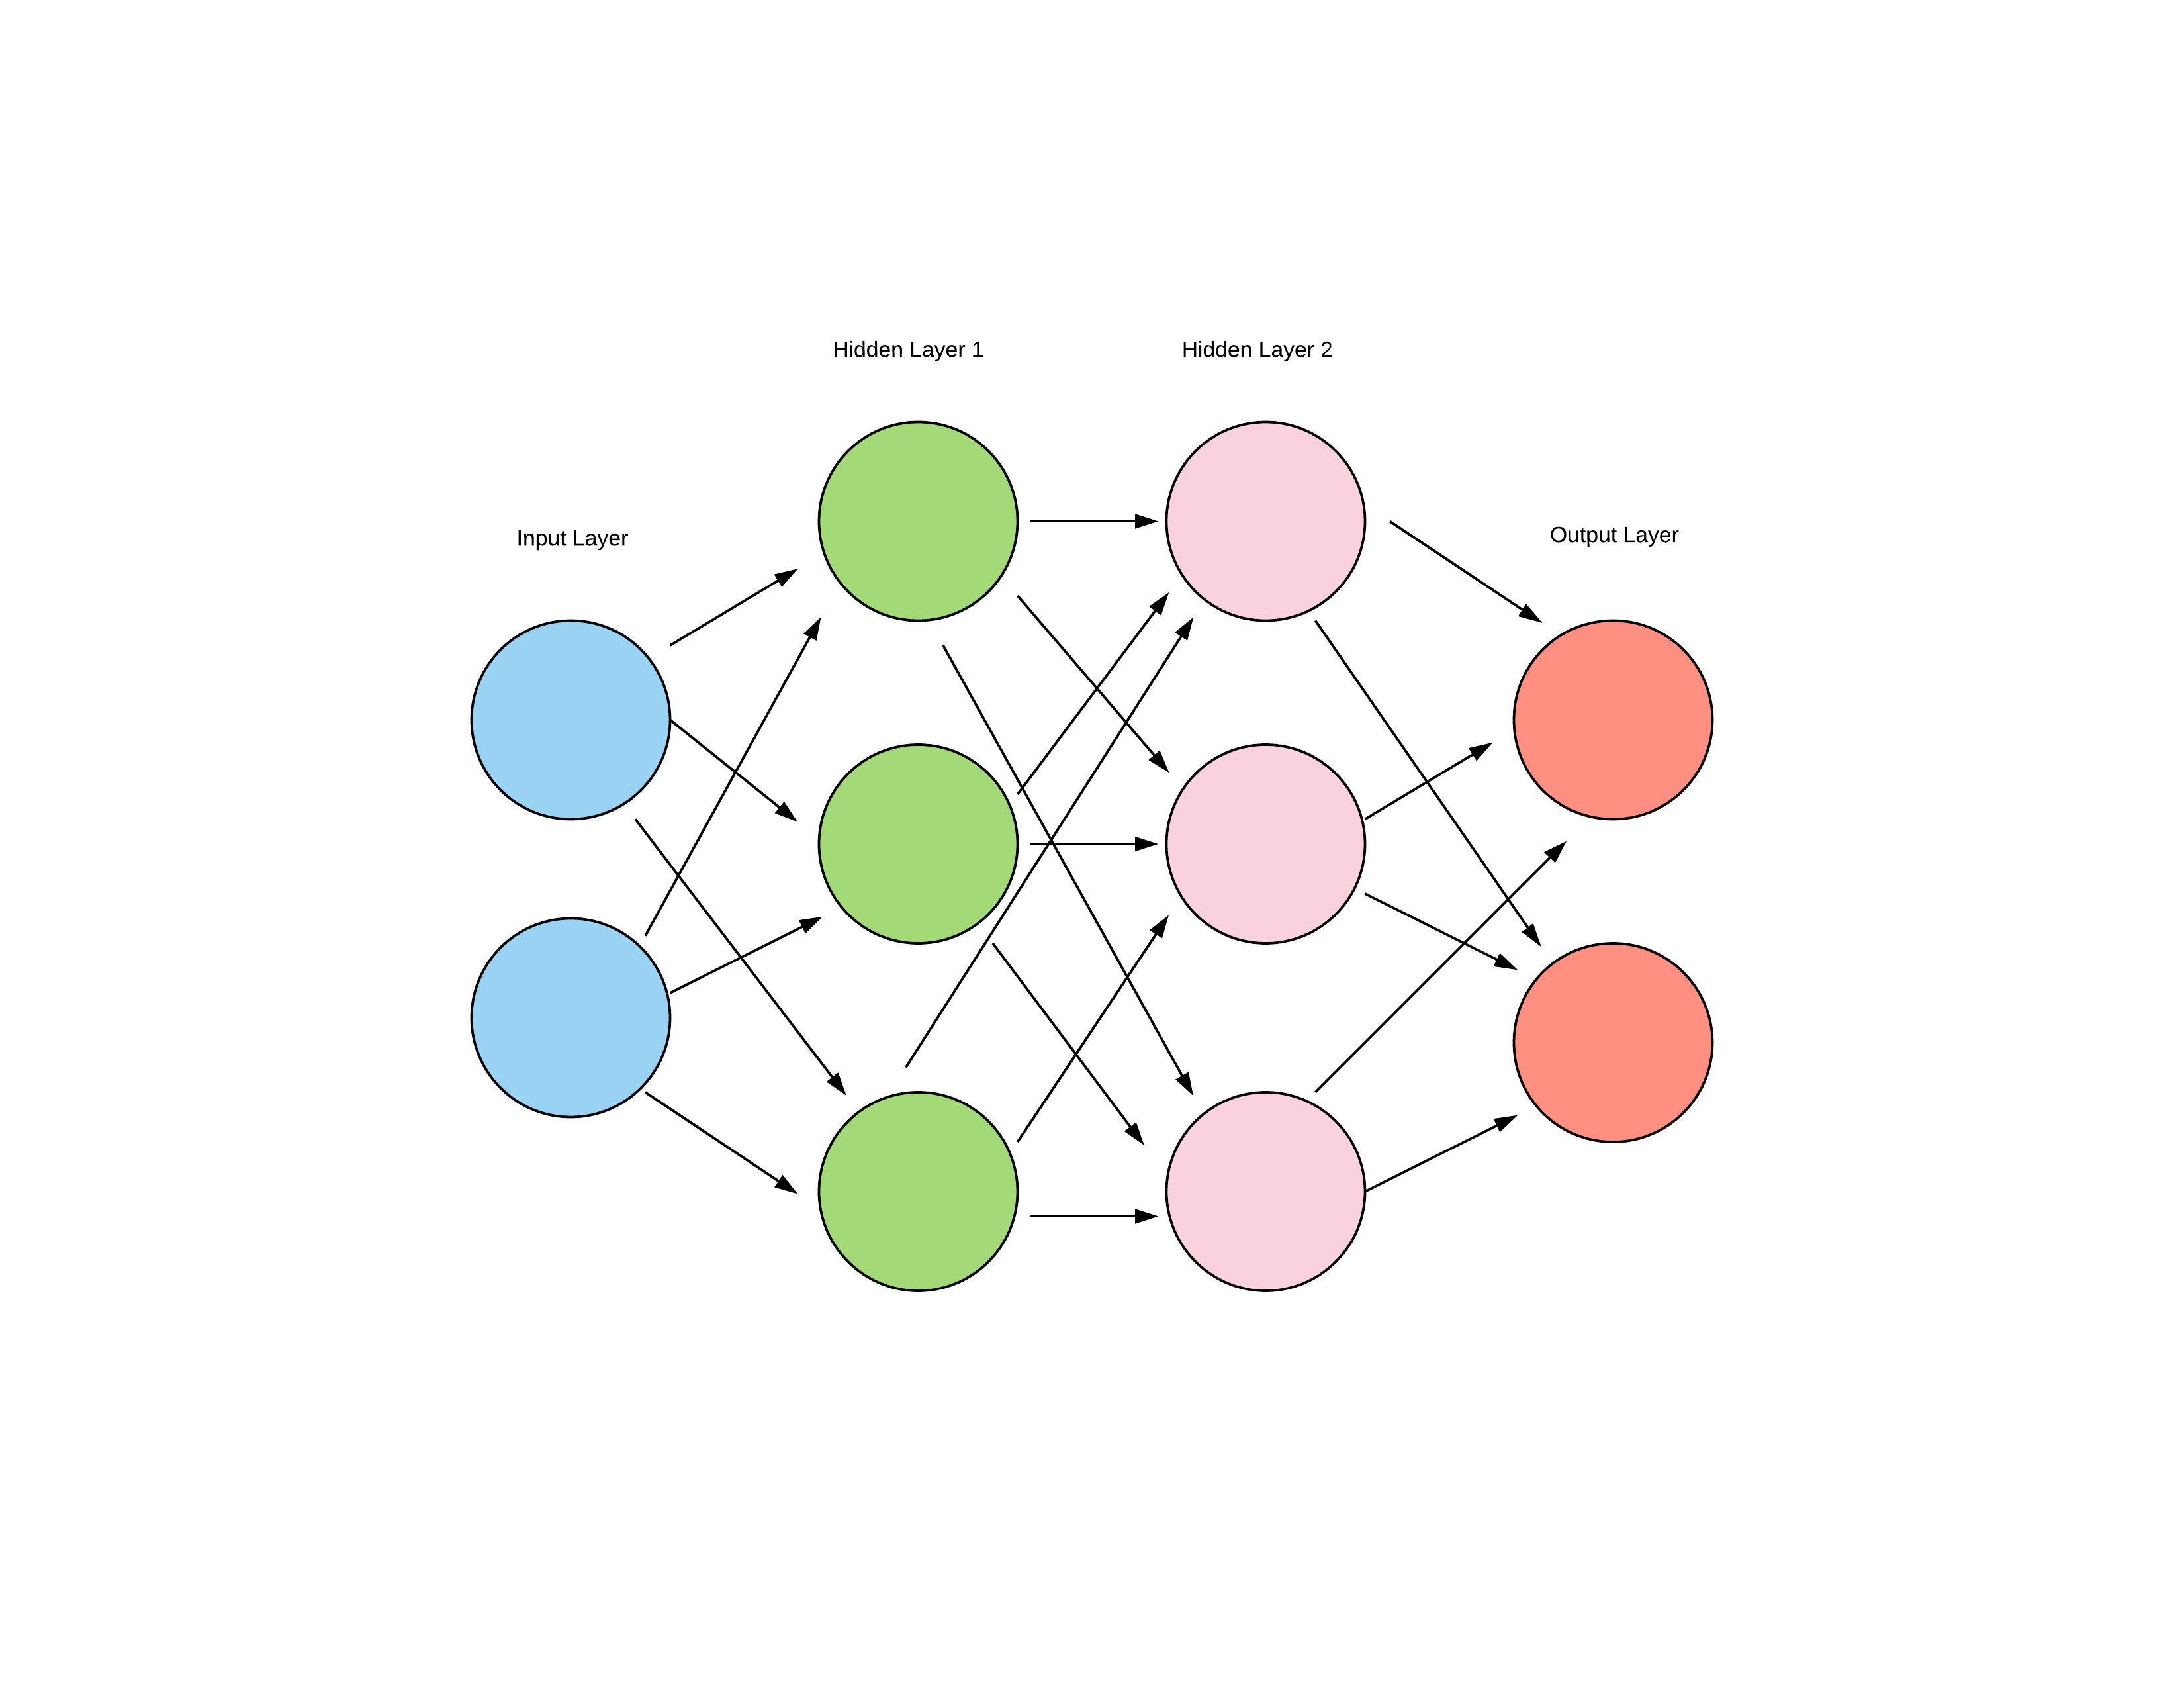
\includegraphics[width=150mm,scale=0.5]{mlp}
    \caption{Multi Layer Perceptron}
    \label{fig:mlp}
\end{figure}

The input layer of a network consists of the data that is fed into the network to be classified. The input layer passes this data to a hidden layer
whose purpose is to transform this data into something that the output layer can
understand. This transformation results in a linearly separable space that can be classified. The output layer normally consists of a class prediction.

MLPs are a class of feed forward ANNs.
These means that the output of each perceptron feeds into an input in the next
layer of the network, example seen in Figure \ref{fig:mlp}.

During training, using backpropagation for each step, the output of every neuron is calculated in each layer and then passed to the next layer. Then the error of the output is calculated, and the network calculates how each neuron in the last hidden layer effected the error. This is continued back through all the layers until the input layer \parencite{handsOnML}. The weights are then altered to try and reduce this error.

There is one large problem with MLP's and as a result CNNs were created. If one is attempting to classify images with a MLP then
each pixel in that image would have to be a separate input. This creates a
massive number of neurons through all the layers and this isn't feasible. CNN's
solve this problem which we will discuss later.

